% section
\section{Image Prediction Architectures} 
 \begin{frame}
  \frametitle{Related work}  
  
  \begin{itemize}
   \item<1-> Description of five state-of-the-art image-/video-prediction architectures
   \item<2-> Different approaches, but all use a LSTM as recurrent sub-module
   \item<3-> Experiments are shown on MovingMNIST \cite{LeCun1998}
  \end{itemize}
 \end{frame}

 % subsection
 \subsection{LSTM Autoencoder}
  % page 1
  \begin{frame}
   \frametitle{LSTM Autoencoder}
   
   \begin{itemize}
    \item<1-> \glqq Unsupervised Learning of Video Representations using LSTMs\grqq by Srivastava et. al. \cite{Srivastava2015}
    \item<2-> Using the standard LSTM from Hochreiter \& Schmidhuber \cite{Hochreiter1997}
    \item<3-> Autoencoder architecture
    \item<4-> Used for future image prediction \& image reconstruction
    \item<5-> Typical baseline for newer, more advanced algorithms
   \end{itemize}
   
  \end{frame}
  % page 2
  \begin{frame}
   \frametitle{LSTM Autoencoder}
   
   \begin{figure}[H]
    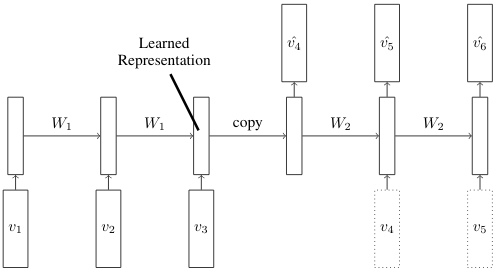
\includegraphics[width=0.7\textwidth]{../Images/srivastava.png}
    \centering
    \caption{Future image prediction model \citep{Srivastava2015}}
    \label{fig:lstm_architecture}
   \end{figure}
  
  \end{frame}
  % page 3
  \begin{frame}
   \frametitle{LSTM Autoencoder}  
  
   \begin{itemize}
    \item<1-> Composed model can do image prediction and reconstruction simultaneously
    \begin{itemize}
     \item<2-> Consisting of one encoder and two decoder
     \item<3-> Good example of representation learning algorithms
     \item<4-> Both use the same encoder but differently trained decoder
    \end{itemize}
    \item<5-> End-to-End differentiable
    \item<6-> Trained with BPTT and CE-Loss for MovingMNIST (two digits per image)
    \item<7-> Used for multi-frame prediction $10$ input images $\Rightarrow$ $10$ output images
   \end{itemize}
  
  \end{frame}
  % page 4
  \begin{frame}
   \frametitle{LSTM Autoencoder}  
  
   \begin{figure}[H]
    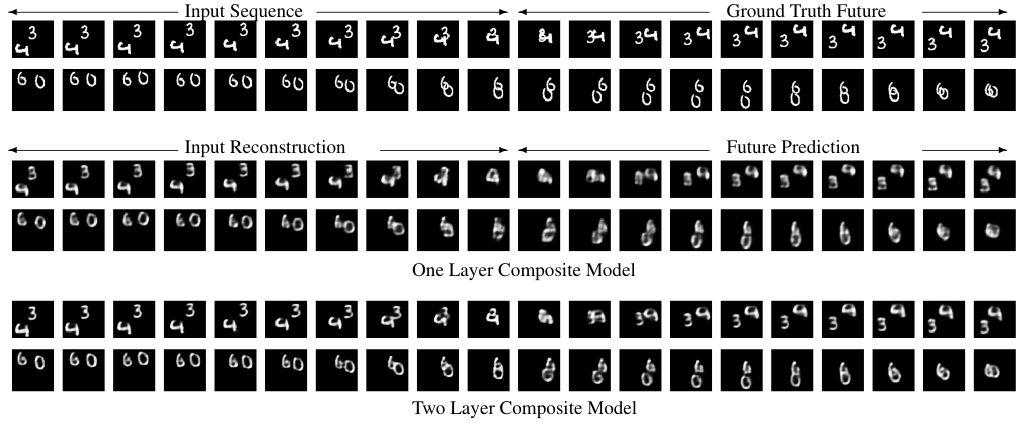
\includegraphics[width=0.7\textwidth]{../Images/srivastava_results_mnist.png}
    \centering
    \caption{Results of MovingMNIST experiment \citep{Srivastava2015}}
    \label{fig:lstm_results_mnist}
   \end{figure}
  
  \end{frame}
 
 % subsection
 \subsection{ConvLSTM Autoencoder}
  % page 1
  \begin{frame}
   \frametitle{ConvLSTM Autoencoder}
   
   \begin{itemize}
    \item<1-> \glqq Convolutional LSTM Network: A Machine Learning Approach for Precipitation Nowcasting\grqq by Shi et. al. \citep{Shi2015}
    \item<2-> Similar to LSTM Autoencoder, but uses novel ConvLSTM instead
    \item<3-> ConvLSTM with peephole connection    
    \item<4-> Outperforms the LSTM Autoencoder \glqq Captures spatiotemporal correlations better\grqq
   \end{itemize}
   
  \end{frame}
  % page 2
  \begin{frame}
   \frametitle{ConvLSTM Autoencoder}
   
   \begin{figure}[H]
    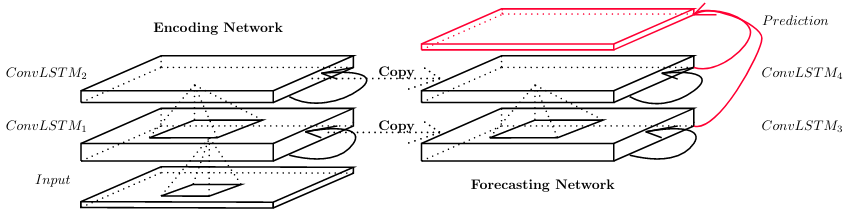
\includegraphics[width=1.0\textwidth]{../Images/shi.png}
    \centering
    \caption{Future image prediction model \citep{Shi2015}}
    \label{fig:convlstm_architecture}
   \end{figure}
   
  \end{frame}
  % page 3
  \begin{frame}
   \frametitle{ConvLSTM Autoencoder}
   
   \begin{itemize}
    \item<1-> End-to-End differentiable
	\item<2-> Trained using BPTT with CE-Loss for MovingMNIST (Three digits per image)
	\item<3-> Used for multi-frame prediction $10$ input images $\Rightarrow$ $10$ output images
	\item<4-> Architecture is only used for forecasting, but might be able to have the same composed model as Srivastava et al. solution
   \end{itemize}
  
  \end{frame}
  % page 4
  \begin{frame}
   \frametitle{ConvLSTM Autoencoder}
   
   \begin{figure}[H]
    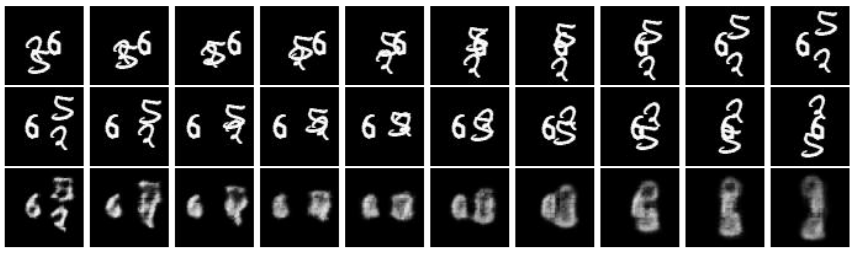
\includegraphics[width=0.7\textwidth]{../Images/shi_results_mnist.png}
    \centering
    \caption{Results of MovingMNIST experiment \citep{Srivastava2015}}
    \label{fig:lstm_architecture}
   \end{figure}  
  
  \end{frame}
 
 % subsection
 \subsection{Spatio-temporal Video Autoencoder}
  % page 1
  \begin{frame}
   \frametitle{Spatio-temporal Video Autoencoder}
   
   \begin{itemize}
    \item<1-> \glqq Spatio-Temporal Video Autoencoder With Differentiable Memory \grqq by Patraucean et. al. \cite{Patraucean2015}
    \item<2-> Using ConvLSTM as recurrent sub-module without peephole connection
    \item<3-> More complex architecture, by nesting an autoencoder inside another
    \begin{itemize}
     \item<4-> The inner autoencoder is for temporal information
     \item<5-> The outer autoencoder is for spatial information
    \end{itemize}
    \item<6-> Spatial autoencoder is a simple undercomplete autoencoder
    \item<7-> Temporal autoencoder consists of a ConvLSTM as temporal encoder and optical flow as temporal decoder
   \end{itemize}
   
  \end{frame}
  % page 2
  \begin{frame}
   \frametitle{Spatio-temporal Video Autoencoder}
   
   \begin{figure}[H]
    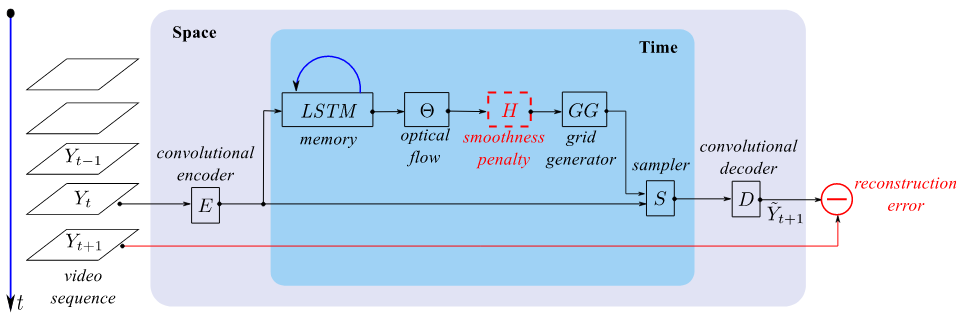
\includegraphics[width=1.0\textwidth]{../Images/patraucean.png}
    \centering
    \caption{Spatio-temporal Video Autoencoder Architecture \citep{Patraucean2015}}
    \label{fig:spatiotemp_architecture}
   \end{figure}
   
  \end{frame}
  \begin{frame}
   \frametitle{Spatio-temporal Video Autoencoder}
   
   \begin{itemize}
    \item<1-> First input the whole image sequence $X$ to the convolutional encoder (Works like a truncated SVD)
    \item<2-> Save the last output of the convolutional encoder
    \item<3-> Use the output sequence of the convolutional encoder as input for the ConvLSTM
    \item<4-> Output of ConvLSTM will get into the optical flow convnet
    \item<5-> Normalize optical flow map and apply with saved image in image sampler
    \item<6-> \glqq Resize\grqq next image.
   \end{itemize}
  
  \end{frame}
  % page 3
  \begin{frame}
   \frametitle{Spatio-temporal Video Autoencoder}
   
   \begin{itemize}
    \item<1-> End-to-End differentiable
	\item<2-> Trained using BPTT with CE-Loss for MovingMNIST (Two digits per image)
	\item<3-> Used for one-frame prediction ($19$ images as input, one as output)
	\item<4-> Architecture could be used for multi-frame prediction with a feedback loop
   \end{itemize}
  
  \end{frame}
  % page 4
  \begin{frame}
   \frametitle{Spatio-temporal Video Autoencoder}  
  
   \begin{figure}[H]
    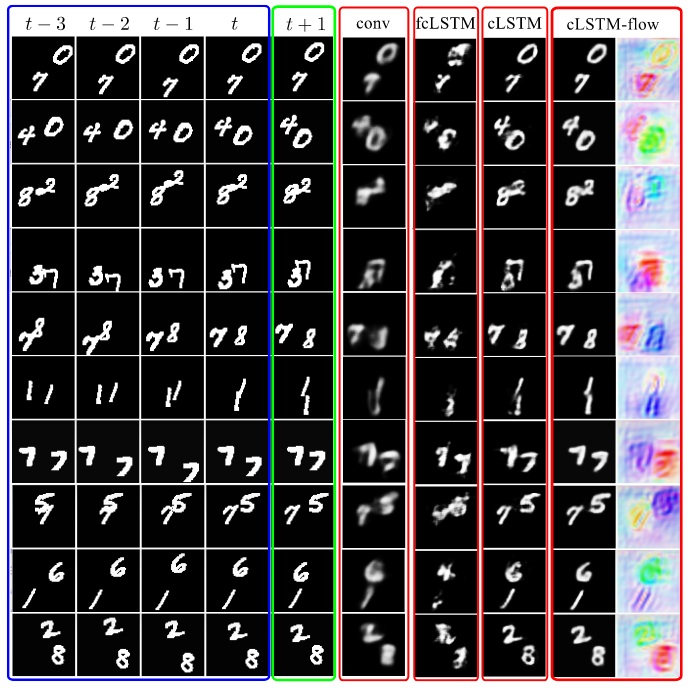
\includegraphics[width=0.55\textwidth]{../Images/patraucean_results_mnist.png}
    \centering
    \caption{Results of MovingMNIST experiment \citep{Patraucean2015}}
    \label{fig:lstm_architecture}
   \end{figure}  
  
  \end{frame}
 
 % subsection
 \subsection{PredNet}
  \begin{frame}
   \frametitle{PredNet}
   
   \begin{itemize}
    \item<1-> \glqq Deep Predictive Coding Networks For Video Prediction And Unsupervised Learning\grqq by Lotter et al. \cite{Lotter2016}
    \item<2-> Informally named PredNet
    \item<3-> Architecture is based on the concept of \glqq predictive coding\grqq.
    \begin{itemize}
     \item<4-> Neuro-scientific task of \glqq continually making predictions of incoming sensory stimuli\grqq.
    \end{itemize}
    \item<5-> Network consists of arbitrary amount of layers
    \item<6-> Depth of network is hyperparameter
   \end{itemize}
   
  \end{frame}
  \begin{frame}
   \frametitle{PredNet}
   
   \begin{figure}[H]
    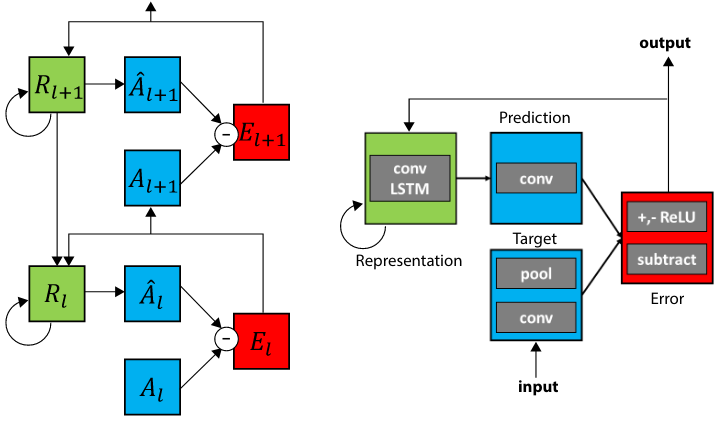
\includegraphics[width=0.8\textwidth]{../Images/lotter.png}
    \centering
    \caption{PredNet Architecture \citep{Lotter2016}}
    \label{fig:spatiotemp_architecture}
   \end{figure}
   
  \end{frame}
  \begin{frame}
   \frametitle{PredNet}
   
   \begin{itemize}
    \item<1->{
     \begin{equation}
      A{_l}^t = \begin{cases} x_t & l = 0 \\ MaxPool(ReLU(Conv(E_{l-1}^t))) & l > 0 \end{cases}
     \end{equation}
    }
    \item<2->{
     \begin{equation}
      \hat{A_l^t} = ReLU(Conv(R_l^t)
     \end{equation}
    }
    \item<3->{
     \begin{equation}
      E_l^t = [ReLU(\hat{A_l^t} - A_l^t); ReLU(A_l^t - \hat{A_l^t})]
     \end{equation}
    }
    \item<4->{
     \begin{equation}
      R_l^t = ConvLSTM(E_l^{t-1}, R_l^{t-1}, Upsample(R_{l+1}^t)
     \end{equation}
    }
   \end{itemize}
   
  \end{frame}
  \begin{frame}
   \frametitle{PredNet}
   
   \begin{itemize}
    \item<1-> Doing prediction in every time-step instead after whole sequence
    \item<2-> First time-step will output a spatially uniform prediction
    \begin{itemize}
     \item<3-> Because $R_l$ and $E_l$ are initialized with zero
    \end{itemize}
    \item<4-> First compute $R_l^t$ states in the top-down pass
    \item<5-> Then compute $\hat{A}_l^t$ in forward pass
    \item<6-> If current layer is $neq$ lowest layer, compute $A_l^t$
    \begin{itemize}
     \item<7-> $A_0^t$ is an image of the input sequence
    \end{itemize}
   \end{itemize}
   
  \end{frame}
  \begin{frame}
   \frametitle{PredNet}
   
   \begin{itemize}
    \item<1-> End-to-End differentiable
    \item<2-> Trained using BPTT
    \item<3-> Using an in-build error function
    \begin{itemize}
     \item<4-> Network consists of two modes (Error and Prediction mode)
     \item<5->{
      \begin{equation}
       L_t = \sum_{t}\lambda_t \sum_l \frac{\lambda_l}{n_l} \sum_{n_l}E_l^t
      \end{equation}     
     }
    \end{itemize}
   \end{itemize}
  \end{frame}
  \begin{frame}
   \frametitle{PredNet}
   
   \begin{figure}[H]
    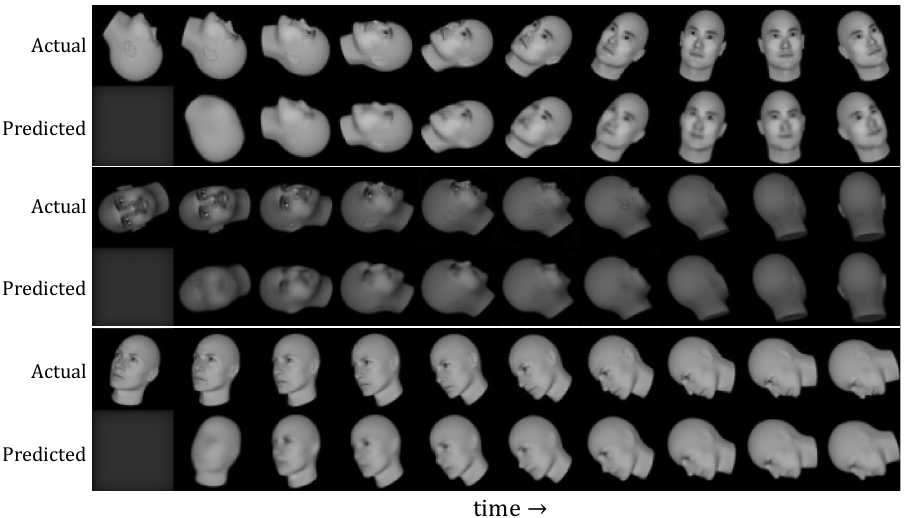
\includegraphics[width=0.8\textwidth]{../Images/prednet.png}
    \centering
    \caption{Results of FaceGen \citep{Lotter2016}}
    \label{fig:facegen_lotter}
   \end{figure}
   
  \end{frame}
  \begin{frame}
   \frametitle{PredNet}
   
   \begin{figure}[H]
   \centering
   \subfloat[Ground truth]{{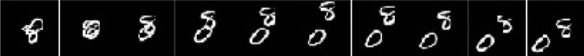
\includegraphics[width=0.75\textwidth]{../Images/prednet_mnist_actual.png} }} 
   \qquad
   \subfloat[ConvLSTM]{{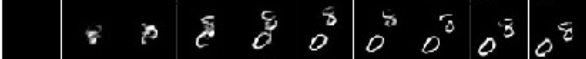
\includegraphics[width=0.75\textwidth]{../Images/prednet_mnist_prediction.png} }} 
   \caption{Results for MovingMNIST \cite{Elsayed2018}.}
   \label{figure::elsayed_mnist}
  \end{figure}
  
  \end{frame}
  
 % subsection
 \subsection{PredRNN}
  \begin{frame}
   \frametitle{PredRNN}
   
   \begin{itemize}
    \item<1-> \glqq PredRNN: Recurrent Neural Networks for Predictive Learning using Spatiotemporal LSTMs\grqq by Wang et al. \cite{Wang2017}
    \item<2-> Novel LSTM module named Spatiotemporal LSTM (ST-LSTM)
    \begin{itemize}
     \item<3-> Consists of the typical temporal memory and extends this with an additional spatiotemporal memory
    \end{itemize}
    \item<4-> Novel Architecture named PredRNN
   \end{itemize}
  
  \end{frame}
  \begin{frame}
   \frametitle{PredRNN}
   
   \begin{equation}
   g_t = tanh(W_{xg} \ast X_t + W_{hg} \ast H_{t-1}^l + b_g)
  \end{equation}
  \begin{equation}
   i_t = \sigma(W_{xi} \ast X_t + W_{hi} \ast H_{t-1}^l +b_i)
  \end{equation}
  \begin{equation}
   f_t = \sigma(W_{xf} \ast X_t + W_{hf} \ast H_{t-1}^l + b_f)
  \end{equation}
  \begin{equation}
   C_t^l = f_t \odot C_{t-1}^l + i_t \odot g_t
  \end{equation}
  \begin{equation}
   g_t\prime = tanh(W_{xg}\prime \ast X_t + W_{mg} \ast M_t^{l-1} + b_g\prime)
  \end{equation}
  \begin{equation}
   i_t\prime = \sigma(W_{xi}\prime \ast X_t + W_{mi} \ast M_t^{l-1} + b_i\prime)
  \end{equation}
  \begin{equation}
   f_t\prime = \sigma(W_{xf}\prime \ast X_t + W_{mf} \ast M_t^{l-1} + b_f\prime)
  \end{equation}
  \begin{equation}
   M_t^l = f_t\prime \odot M_t^{l-1} + i_t\prime \odot g_t\prime
  \end{equation}
  \begin{equation}
   o_t = \sigma(W_{xo} \ast X_t + W_{ho} \ast H_{t-1}^l + W_{co} \ast C_t^l + W_{mo} \ast M_t^l + b_o)
  \end{equation}
  \begin{equation}
   H_t^l = o_t \odot tanh(W_{1 \times 1} \ast [C_t^l, M_t^l])
  \end{equation}
   
  \end{frame}
  \begin{frame}
   \frametitle{PredRNN}
   
   \begin{figure}[H]
    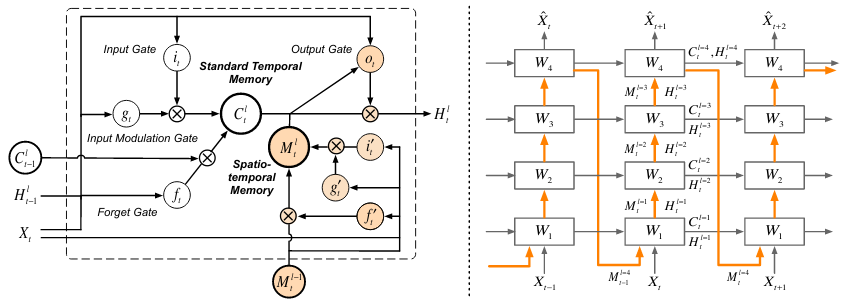
\includegraphics[width=0.8\textwidth]{../Images/wang.png}
    \centering
    \caption{\textbf{Left:} ST-LSTM architecture, \textbf{Right:} PredRNN architecture \cite{Wang2017}}
    \label{fig:wang_architecture}
   \end{figure}
   
  \end{frame}
  \begin{frame}
   \frametitle{PredRNN}
   
   \begin{itemize}
    \item<1-> End-to-End differentiable
    \item<2-> Trained using BPTT using CE-Loss on MovingMNIST (Two digits per frame)
    \item<3-> Using ten images as input and output ten images
   \end{itemize}      
   
  \end{frame}
  \begin{frame}
   \frametitle{PredRNN}
   
   \begin{figure}[H]
   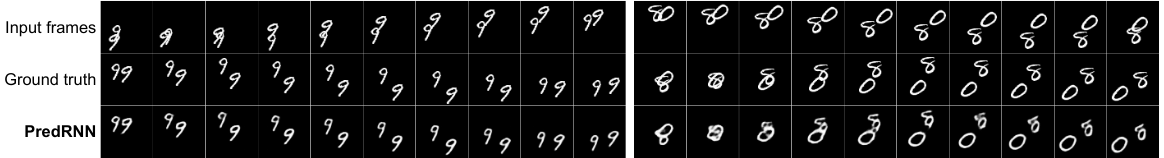
\includegraphics[width=1.0\textwidth]{../Images/predrnn_mnist.png}
   \centering
   \caption{Results for MovingMNIST \cite{Wang2017}.}
   \label{fig:predrnn_mnist}
  \end{figure}   
   
  \end{frame}
  
 \begin{frame}
  \frametitle{Related work}
  
  \begin{itemize}
   \item<1-> Architectures have different approach but similar result
   \item<2-> First architecture uses LSTM in autoencoder architecture
   \item<3-> The second architecture replaces the LSTM with ConvLSTM
   \item<4-> Third architecture leverages optical flow with two autoencoder, two split information in space and time
   \item<5-> PredNet introduces a neuro-scientific idea to achieve state-of-the-art image-/video-prediction
   \item<6-> The last architecture introduces a novel ConvLSTM named ST-LSTM and also a novel architecture named PredRNN
   \item<7-> $\Rightarrow$ Even though, the algorithms have different approaches to perform state-of-the-art image-/video-prediction, they all use some kind
   of LSTM as recurrent module.
  \end{itemize}
 \end{frame}
